\chapter{Results and Evaluation}

In section \ref{desired_outcomes} on page \pageref{desired_outcomes}, the desired outcomes of the project are described. This chapter critically assesses to what extent these outcomes have been met.

\section{Verifying Bias in Test Train Split}

This section examines the limitations of the evaluation. This is done by measuring the bias in the data, using k-folds cross-validation, shuffle split and hold-out testing.

Note that not all types of bias, such as selection bias, can be measured this way and therefore the impact of these biases remains unknown.

\subsection{Quantifying Bias}

Bias in evaluation is inevitable. In section \ref{sub: data_prep} on page \pageref{sub: data_prep} we specified that the data is shuffled to eliminate ordering bias. However, shuffling the data introduces random bias. 

By using k-folds cross-validation we can generate 5 confusion matrices for each model, one for each k-fold, and then we can measure the standard deviation in the confusion matrix metrics.

Table \ref{tbl:x kf_std_cm} on page \pageref{tbl:x kf_std_cm} shows the mean standard deviation of the true positive and false negative metric between the 5 train test splits is 4.1e-03 and 3.39e-03 respectively. This is equivalent to 0.41\% and 0.39\% standard deviation.

For the purpose of evaluating the models in this project, this deviation between splits is considered insignificant. Therefore evaluations are made on one of the k-fold test train subsets, k1.

\begin{table}
    \centering
    \begin{tabular}{c c c} 
         \toprule
         Model & True Positive $\sigma$ & True Negative $\sigma$ \\
         \midrule
         model3 & 1.75e-03 & 5.36e-04\\
         model4 & 1.78e-03 & 8.51e-04\\ 
         model5 & 1.73e-03 & 1.14e-03\\
         model6 & 4.07e-03 & 3.27e-03\\
         model7 & 2.15e-03 & 4.2e-03\\
         model8 & 1.54e-03 & 3.32e-03\\ 
         model9 & 2.21e-02 & 1.71e-02\\
         model10 & 2.27e-03 & 1.45e-03\\
         model11 & 1.95e-03 & 1.41e-03\\
         model13 & 1.64e-03 & 6.36e-04\\
         model14 & 2.182838e-03 & 6.061164e-04\\
         \hline
         \textbf{mean} & 4.1e-03 & 3.39e-03 \\
         \bottomrule
    \end{tabular}
    \caption{Standard deviation of specificity and sensitivity across each test train split}
    \label{tbl:x kf_std_cm}
\end{table}

\newpage

\section{Desired Outcome 1: Evaluating iArsenic Models}

This section details how desired outcome 1 has been achieved. See the desired outcomes at \ref{desired_outcomes} on page \pageref{desired_outcomes}

Table \ref{tbl:x model_evals} on page \pageref{tbl:x model_evals} shows evaluation metrics of the iArsenic and the machine learning based models, and chart \ref{fig:x mpf1} on page \pageref{fig:x mpf1} shows the f1 scores in this table as a bar chart.

The iArsenic models, model3, model4 and model5, have been developed sequentially with each model improving on the one before. The evaluations show that the models have been improving with each iteration. The evaluation also shows that the best performing iArsenic model, model5, achieved an accuracy of 84\% and an f1 of 82\% and a true negative rate of 85\%. See \ref{fig:x Confusion Matrix mode5 Red Staining} on page \pageref{fig:x Confusion Matrix mode5 Red Staining} for a confusion matrix of model5.

Compared to the other models in the literature review, this appears to be a very high level of performance. Though further analysis is required to confirm this as an evaluation metric common to each of these models must be identified. 

\subsection{Benefit of Evaluation of iArsenic Models}

Evaluating the iArsenic models validates their performance and quantifies their suitability for implementation in the iArsenic web application. This facilitates a more informed application of predictions from these models.

The evaluation shows that the performance of the models is increasing with each iteration from model3 to model5, indicating that performance has not plateaued so the development of further models may produce further improvements in performance.

If new iArsenic models are developed, the evaluation of the existing models will be able to indicate where the existing models are underperforming, aiding the development of new models.

The benefit of this evaluation supports the notion that geoscientists should about learn machine learning and artificial intelligence, as the tools and techniques required to generate this kind of evaluation are core in the field of machine learning. 

\subsection{Desired Outcome Achievement}

Prior to this project, there was no evaluation of the iArsenic models. While each iteration was more sophisticated than the last and was presumed to perform better, this was not verifiable.

Because of the evaluations done in this project, it is now verifiable that the models do perform well.

The confusion matrices produced for each model offer a detailed evaluation of the performance of each model. While other evaluation techniques such as receiver operator curves were considered, not all models were able to generate them.

Confusion matrix metrics are displayed in table \ref{tbl:x model_evals} on page \pageref{tbl:x model_evals}.

\newpage

\section{Desired Outcome 2: Comparing iArsenic to Machine Learning Models}

\cite{Fleming2021} makes the case that because of the prevalence of artificial intelligence in earth and environmental science, earth and environmental science students should be taught machine learning and artificial intelligence skills to give geoscientists the ability to work with machine learning concepts more effectively than they currently do, usually with self taught skills.

This project provides an opportunity for a case study wherein existing expert system models, developed by the geoscientist Dr Mohammed Hoque for iArsenic, are compared with machine learning based models.

This section will analyse the benefits and limitations machine learning has brought to iArsenic throughout the development of this project.

\subsection{iArsenic \& Machine Learning Models Performance}

By f1 score, the best performing iArsenic model, model5, achieves a score of 82\%. The best machine learning model is model6, with an f1 score of 72\%. This demonstrates that machine learning models do not inherently produce better performance than expert system models.

This indicates that the models made by a geoscientist without a background in machine learning outperformed machine learning based models. This could indicate that geoscientists may not benefit from machine learning and artificial intelligence education.

\subsection{Desired Outcome Achievement}

The development and comparison of iArsenic models to machine learning models show that machine learning models are able to produce generalised predictions. This proves that machine learning models are applicable to the iArsenic dataset in a comparable way to the existing models. It is probable that with further work machine learning models, like the ones developed in this project, could outperform the existing models. 

\section{Conclusion}

Evaluating the iArsenic models and comparing them to machine learning based models has been a success.

The evaluation of the iArsenic models is a valuable contribution to the application and development of the iArsenic models and iArsenic more broadly. The tools and techniques required to generate these evaluations are rooted in machine learning and artificial intelligence. It could be argued, specifically in the case of iArsenic, that if these skills were more prevalent in geoscience, this would provide a significant benefit. This reinforces the case made in \cite{Fleming2021}.

This project also shows that machine learning is no silver bullet. While the benefit of evaluation is clear, the best performing models in this project were developed specifically from a geoscience background. Indicating that machine learning is not required by geoscientists to make predictive models. This arguably weakens the case made in \cite{Fleming2021}, though with refinement it is possible that machine learning based models could perform at least as well as the expert models, especially if more sophisticated model frameworks are considered.

To conclude, while machine learning skills are valuable, increasing collaboration between geoscience and computer science may be a more practical route to the same effect as increasing machine learning education in geoscience.

\begin{figure}[h]
    \centering
    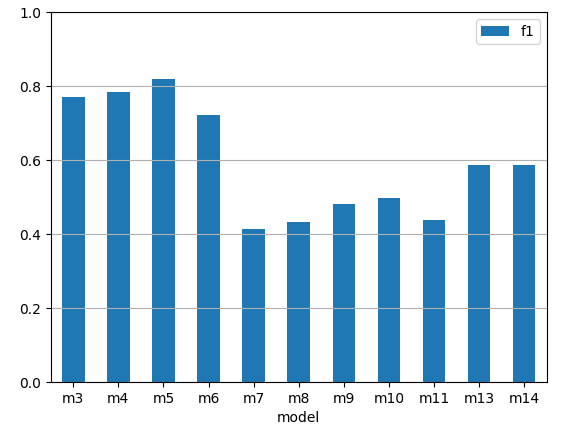
\includegraphics[scale=0.6]{figures/model_f1_barchart.png} 
    \caption{Model performance by f1 score}
    \label{fig:x mpf1}
\end{figure}

\begin{table}
    \centering
    \begin{tabular}{c c c c c c} 
         \toprule
         Model & True Positive & True Negative & f1 & accuracy & precision\\
         \midrule
         model3 & 0.719387 & 0.880010 & 0.771552 & 0.807386 & 0.831874\\
         model4 & 0.741016 & 0.876879 & 0.784060 & 0.815450 & 0.832413\\ 
         model5 & 0.814367 & 0.854302 & 0.818085 & 0.836246 & 0.821837\\
         model6 & 0.725523 & 0.763088 & 0.720984 & 0.746103 & 0.716502\\
         model7 & 0.378534 & 0.623378 & 0.412596 & 0.512674 & 0.453395\\
         model8 & 0.414230 & 0.587080 & 0.432714 & 0.508927 & 0.452924\\
         model9 & 0.410958 & 0.753969 & 0.480913 & 0.598880 & 0.579569\\
         model10 & 0.447443 & 0.706891 & 0.497044 & 0.589187 & 0.559013\\
         model11 & 0.421738 & 0.579780 & 0.437537 & 0.508081 & 0.454565\\
         model13 & 0.663838 & 0.503931 & 0.585893 & 0.576156 & 0.524328\\
         model14 & 0.663940 & 0.503868 & 0.585936 & 0.576167 & 0.524335\\
         \bottomrule
    \end{tabular}
    \caption{Table of evaluation metrics for all models}
    \label{tbl:x model_evals}
\end{table}